\documentclass{article}
\usepackage{graphicx} % Required for inserting images
\usepackage{pdflscape}
\usepackage{multicol}
\usepackage{amsmath}
\usepackage{amssymb}
\usepackage{fancyhdr}
\usepackage{cancel}
\usepackage{tgbonum}
\usepackage{float}
\usepackage[swedish]{babel}
\usepackage{hyperref}
\usepackage{wasysym}
\usepackage{enumitem}
\usepackage{tabularx}
\usepackage[title]{appendix}
\usepackage[dvipsnames]{xcolor}\usepackage{tgadventor}
\usepackage{helvet}
 \usepackage[stable]{footmisc}
\usepackage{parskip}
\usepackage[swedish]{babel}
\usepackage{dirtytalk}
\usepackage[a4paper, landscape]{geometry}
\renewcommand{\headrule}{}
 \renewcommand{\familydefault}{phv}
\usepackage{sectsty}
\allsectionsfont{\fontfamily{qag}\selectfont}
\pagestyle{fancy}
\pagecolor{SkyBlue!10}
\fancyhf{}
\fancyhead[C]{
\fontfamily{cmr}\selectfont
\colorbox{yellow!25!white}{
\makebox[\textwidth]{
\large{
\llap{\textbf{Mekanik I - Sammanfattning}$\quad\cdot$}
\clap{}
\rlap{\textit{Albin Seijmer}$\cdot$\textit{COPEN}}
}
}
}
\color{ProcessBlue}\rule{\textwidth}{2pt}
}
\newcommand{\dummyargument}{}
\newenvironment{ankiflashcard}[1]{}{}
\usepackage{blindtext}
\usepackage{paracol}
% Column configuration
\setlength{\columnsep}{2em}
\setlength{\columnseprule}{0.1pt}
% Row configuration for tables and arrays
\renewcommand{\arraystretch}{1.25}
\usepackage{amsmath}
\setcounter{secnumdepth}{0}
\title{Mekanik I - Sammanfattning}
\date{}
% Own commands
\newcommand{\ruler}{
\rule{0.5\textwidth}{0.5pt}
}
\newcommand{\numbercircle}[1]{
\text{\textcircled{#1}}
}
\newcommand{\numbercirclewithunderbrace}[2]{
\underbrace{#1}_{\numbercircle{#2}}
}
\usepackage{tikz}

\newcommand\centerofmass{%
    \tikz[radius=0.4em] {%
        \fill (0,0) -- ++(0.4em,0) arc [start angle=0,end angle=90] -- ++(0,-0.8em) arc [start angle=270, end angle=180];%
        \draw (0,0) circle;%
    }%
}
\newcommand{\midtitle}[1]{
\begin{center}
\Huge{\text{#1}}
\newpage
\end{center}
}
\begin{document}
\Huge{Mekanik I - Sammanfattning}
\large\newline
\textit{Med reseveration för att formler och/eller fakta är felaktiga och övriga skrivfel. Den senaste versionen av formelbladet (tillsammans med flashcards) finns att hitta, free of charge, no strings attached, på \url{https://github.com/sotpotatis/mekanik-i-cheatsheet}. \textbf{Lycka till!}}
\newpage
\midtitle{Statik}
\begin{paracol}{2}
\section{Vektoralgebra}
\subsection{Enhetsvektor}
För att göra en vektor till en enhetsvektor (längd $1$):
$$
\boxed{
\vec v = \frac{1}{\left\| \vec v \right\|} \cdot \vec v
}
$$
\subsection{Skalärprodukt}
\subsubsection{Skalärproduktens samband med vinkeln:}
$$
\boxed{
(\vec a \cdot \vec b)=\left\|a\right\|\left\|b\right\|\cos\alpha
}
$$
\subsubsection{Projektion på enhetsvektor}
Storleken av projektionen av en godtycklig vektor $\vec a$ på $\vec b$ ges av formeln för vinkeln ovan.
Projicera $\vec a$ på enhetsvektorn $\hat e_v$ 
$$
proj_{\hat e_v}(\vec a)=(\vec a \cdot \hat e_v)\cdot \hat e_v
$$
observera att har vi en enhetsvektor gäller
$$
(\vec a \cdot \hat e_v)=\left\|a\right\|cos\alpha
$$
$\alpha$ är vinkeln mellan vektorerna.

\subsection{Vektorkomponenter}
Se bild.
$$
\begin{cases}
a_x = acos\alpha\\
a_y = acos\beta\\
a_y = acos\gamma
\end{cases}
$$
\subsection{Kryssprodukt}
\subsubsection{Kryssproduktens samband med vinkeln:}
$$
\boxed{
\left\|\vec a \times \vec b \right\|=\left\|\vec a \right\|\left\|\vec b \right\|sin\alpha
}
$$

\subsubsection{Räkneregler \& area:}
Observera att \textit{kryssproduktens belopp=arean som spänns upp av } $\vec a$ \& $\vec b$


Kryssprodukten är inte kommutativ: $\vec a \times \vec b = -\vec b \times \vec a$

\subsubsection{Determinant-minnesregel för kryssprodukten:}
$$
\vec a \times \vec b =
\begin{bmatrix}
\hat e_1&\hat e_2&\hat e_3\\
a_x&a_y&a_z\\
b_x&b_y&b_z\\
\end{bmatrix}
$$
\subsubsection{Högerhandsregeln för kryssprodukt:}
\begin{itemize}
    \item Rikta alla fingrar utom tummen längs med första vektorn ($\vec a$).
    \item  Skruva fingrarna i riktning mot andra vektorn ($\vec b$)
    \item Tummen pekar i riktningen $\vec a\times\vec b$.
    
\end{itemize}

% DONOTREMOVE ANKI-FLASHCARD GUID 1243539431
\begin{ankiflashcard}{Ange formeln för dubbla kryssprodukten.}
\subsubsection{Dubbla kryssprodukten:}
$$
\vec a \times \vec b \times \vec c =\vec b(\vec a \times \vec c)-\vec c(\vec a \cdot \vec b)
$$
\end{ankiflashcard}

\section{Olika typer av kraftsystem}

% DONOTREMOVE ANKI-FLASHCARD GUID 1190208710
\begin{ankiflashcard}{Vad är ekvivalenta kraftsystem? Vad kännetecknas de av?}
\subsection{Ekvivalenta kraftsystem}
Relation mellan två system där kraftsumman \textit{och} momentsumman är densamma.
\ruler
\end{ankiflashcard}

% DONOTREMOVE ANKI-FLASHCARD GUID 1526209209
\begin{ankiflashcard}{Vad är ekvimomenta kraftsystem? Vad kännetecknas de av?}
\subsection{Ekvimomenta kraftsystem}
Ett system där:
\begin{enumerate}
    \item Kraftsumman är samma
    \item Momentsumman är samma i \underline{en} punkt.
\end{enumerate}
$\rightarrow$ \underline{Ekvimomenta} kraftsystem är \underline{ekvivalenta}.
\end{ankiflashcard}

% DONOTREMOVE ANKI-FLASHCARD GUID 1549934742
\begin{ankiflashcard}{Vad är ett kraftpar, och vad kännetecknar kraftparet?}
    
\subsection{Kraftpar}
Kraftpar är ett kraftsystem som består av två lika stora och motriktade krafter.
\textbf{Kraftsumma:} $0$.


\textbf{Momentsumma:} oberoende av punkt.


Notera även att $\left\lvert M_O \right\rvert = Fh\quad\left\{\begin{array}{l}M_O: \text{Momentet i origo} \\F: \text{Beloppet av kraften i systemet} \\h: \text{Avstånd mellan krafterna} \\\end{array}\right.$
eller på vektorform: $\vec{r_{BA}} = M_O \times F_1$
\end{ankiflashcard}

% DONOTREMOVE ANKI-FLASHCARD GUID 1730687558
\begin{ankiflashcard}{Ange formeln och definitionen för reduktionsresultat.}
\subsection{Reduktionsresultatet}
Innebär att vi \textit{reducerar} ett komplext kraftsystem till att bestå bara av \textit{\underline{en} kraft} och \textit{\underline{ett} moment}. Resultatet kallas ett reduktionsresultat med avseende på en punkt $P$.
\end{ankiflashcard}

% DONOTREMOVE ANKI-FLASHCARD GUID 1756469926
\begin{ankiflashcard}{Ange formeln för erättningsmoment}
Varje gång vi flyttar en kraft för att reducera kraftsystemet, måste vi lägga till ett moment för att  kompensera för flytten, ett \newline
\textbf{ersättningsmoment:}
$$
\vec M_A = \vec{r_{AP}} \times \vec F
$$
Se figur nedan för beteckningar:
\begin{figure}[H]
    \centering
    \includegraphics[width=5cm]{ersättningsmoment.png}
    \caption{Ersättningsmoment}
\end{figure}
\end{ankiflashcard}

% DONOTREMOVE ANKI-FLASHCARD GUID 1590469722
\begin{ankiflashcard}{Definera kraftsumma och momentsumma vid reduktionsresultat.}
Om vi flyttar alla krafter till samma punkt, får vi en \textbf{total kraftsumma vid reduktionsresultat:}
$$
\vec F = \overset{n}{\underset{n=1}{\sum}} \vec F_n
$$
Vi får också en en \textbf{total momentsumma vid reduktionsresultat:}
$$
\vec M = \overset{n}{\underset{n=1}{\sum}} \vec{r_{AP_n}} \times \vec{F_n}
$$
\fbox{
\begin{minipage}{0.45\textwidth}
\textit{Observera} att den totala kraftsumman generellt inte är vinkelrät mot momentsumman,

\textit{och} att \textit{alla kraftsystem kan reduceras till en kraft och ett moment} (se även \textit{Kraftskruv}).
\end{minipage}
}

\end{ankiflashcard}


% DONOTREMOVE ANKI-FLASHCARD GUID 1539929808
\begin{ankiflashcard}{Ange formeln för flytt av reduktionsresultat.}
    \textit{Flytt av reduktionsresultat} ger att momentsumman ändras enligt \textbf{sambandsformeln:}
$$
\vec M_B = \vec M_A + \vec{r_{BA}} \times \vec F\left\{\begin{array}{l}\vec M_B: \text{Momentet i ny punkt} \\\vec M_A: \text{Moment i tidigare punkt} \\\vec r_{BA}: \text{Avstånd mellan tidigare och ny punkt} \\\vec F: \text{Ersättnings-/reduktionskraft} \\\end{array}\right.$$
\end{ankiflashcard}
\ruler

\section{Pappus regler}
Pappus regler kan användas för att förenkla integraler över masscentrum.

% DONOTREMOVE ANKI-FLASHCARD GUID 1846629937
\begin{ankiflashcard}{Formulera Pappus arearegel.}
\subsection{Pappus arearegel}
Gäller för en massbelagd kurva $\mathcal C$ som ligger på $xy$-planet.
$$
A=2\pi y_G l\\ \implies y_G = \frac{A}{2\pi l}\left\{\begin{array}{l}A: \text{Area av yta efter rotation} \\y_G: \text{y-komponenten för masscentrum} \\l: \text{Längd av kurvan} \\\end{array}\right.
$$
\textit{Notera} att $A$ är botten-/mantelarean som den yta som bildas om du tänker dig att du skapar en rotationsvolym av din kurva.
Exempel: du använder Pappus arearegel för en halvcirkelbåge. Då är rotationsarean en sfär, så $A = 4\pi r^2$. $l$ är däremot längden på din halvcirkel, dvs. $2\pi r$
\textit{Notera även} att denna regel appliceras genom att du i de praktiska fallen söker $y_G$.
\end{ankiflashcard}

% DONOTREMOVE ANKI-FLASHCARD GUID 1585744448
\begin{ankiflashcard}{Formulera Pappus volymregel.}
    \subsection{Pappus volymregel}
Samma koncept som arearegeln, gäller en massbelagd yta med arean $A$.
$$
V = 2\pi y_G A\\
\implies y_G = \frac{V}{2\pi A}
$$
\textit{Notera} att $A$ är arean av den yta som du roterar, och $V$ är volymen som bildas om du tänker dig att du skapar en rotationsvolym av din kurva.
(\textit{skillnad från arearegeln!})
Exempel: du använder Pappus arearegel för en halvcirkel\textit{skiva}. Då är rotationsvolymen en sfär, så $V = 4\pi r^3$. $A$ är däremot arean för din halvcirkelskiva, dvs. $\frac{\pi r^2}{2}$


\textit{Notera även} att även denna regel appliceras genom att du i de praktiska fallen söker $y_G$.
\end{ankiflashcard}

\ruler
\section{Friläggning}
Konceptet av friläggning handlar om att välja hur man ska dela upp ett problem i olika delsystem.

    
\subsection{Frihetsgrader}
% DONOTREMOVE ANKI-FLASHCARD GUID 2109155662
\begin{ankiflashcard}{Vilka frihetsgrader finns i 3D?}
\subsubsection{Frihetsgrader i 3D}

\begin{enumerate}[label*=\protect\fbox{\arabic{enumi}}]
\item translation kring x-axeln
\item translation kring y-axeln
\item translation kring z-axeln
\item rotation kring x-axeln
\item rotation kring y-axeln
\item rotation kring z-axeln
\end{enumerate}
\textit{Notera:} translation betyder att man kan röra sig i ``rymden`` (dvs. koordinatsystemet)
\end{ankiflashcard}

% DONOTREMOVE ANKI-FLASHCARD GUID 1293290979
\begin{ankiflashcard}{Vilka frietsgrader finns i 2D?}
    
\subsubsection{Frihetsgrader i 2D}
\begin{enumerate}[label*=\protect\fbox{\arabic{enumi}}]
\item translation kring x-axeln
\item translation kring y-axeln
\item rotation kring z-axeln
\end{enumerate}
\textit{Notera:} se ovan för information om vad translation betyder.
\end{ankiflashcard}
    
\section{Friktion}
Friktionskraften är en kraft som uppkommer i kontakt mellan två ytor och är parallell med ytan där friktionen uppstår.

% DONOTREMOVE ANKI-FLASHCARD GUID 1958068440
\begin{ankiflashcard}{Ange formeln/definitionen för friktionskraft.}
\subsection{Friktionskraft}
Maximala friktionskraften ges av
$$
F \leq \mu_k N
$$
där $N$ är nomalkraften.
\subsection{Friktionstal}
Det finns ett statiskt friktionstal och ett kinematiskt friktionstal, dock kan man förutsätta att $\mu_s \approx \mu_k \approx \mu$. $\mu_k$ är friktionstalet där glidning börjar inträffa.
\end{ankiflashcard}

% DONOTREMOVE ANKI-FLASHCARD GUID 2067580333
\begin{ankiflashcard}{Ange jämviktsvillkor (friktion)}
\subsection{Jämvikt och glidning}
Om friktionskraftens storlek är enligt
$$
0\leq F \leq \mu_s N \approx \mu N
$$
gäller så har vi \textit{jämvikt}. \textbf{Observera} alltså att storleken på kraften är variabel!
\end{ankiflashcard}

% DONOTREMOVE ANKI-FLASHCARD GUID 1669719265
\begin{ankiflashcard}{Ange glidningsvillkor (friktion)}
Vid $$F=\mu_kN$$ så börjar vi ha \textit{glidning}. Dvs. när
$$
F > \mu_k N \approx \mu N
$$
\end{ankiflashcard}

% DONOTREMOVE ANKI-FLASHCARD GUID 1384999898
\begin{ankiflashcard}{Ange själpningsvillkor (friktion)}
\subsubsection{Stjälpningsvillkor}
Normalkraften på ett objekt kan angripa utanför objektet. Det går alltså att formulera villkoret 
$$r_N\leq L$$
där $r_N$ är avståndet mellan objektets hörn till normalkraften, och $L$ är den maximala längden från hörnet som normalkraften kan röra sig på.
\end{ankiflashcard}
\switchcolumn

% DONOTREMOVE ANKI-FLASHCARD GUID 1131365315
\begin{ankiflashcard}{Hur definieras moment? (generella definitionen)}
\section{Moment}
\subsection{Allmän formel}
Momentet för en kraft i en punkt $A$:
$$
\vec M_P = \vec r_{OA} \times \vec F\quad\left\{\begin{array}{l}\vec M: \text{Moment} \\\vec r_{OA}: \text{Radie från origo till punkten A} \\\vec F: \text{Kraft} \\\end{array}\right.$$
Observera att i $\mathbb R^2$ gäller att
$$
M = Fd
$$
där $d$ är det \textit{vinkelräta avståndet} (hävarmen) som kraften har på momentpunkten.

    
\end{ankiflashcard}

% DONOTREMOVE ANKI-FLASHCARD GUID 1754604283
\begin{ankiflashcard}{Hur definieras momentet med avseende på en axel?}
    
\subsection{Moment med avseende på en axel}
$$
\vec M_{\lambda} = \vec M_P \cdot \hat {e_{\lambda}}\quad\left\{\begin{array}{l}\vec M_{\lambda}: \text{Moment med avsikt på axeln }\lambda \\\vec M_P: \text{Moment i punkten (se ovan)} \\\hat e_\lambda: \text{Enhetsvektor för axeln } \lambda \\\end{array}\right.$$
\textbf{Observera: } momentet med avseende på en axel är en \textit{skalär}!
\end{ankiflashcard}

% DONOTREMOVE ANKI-FLASHCARD GUID 1660318753
\begin{ankiflashcard}{Vad finns för generella regler kring moment?}
\subsection{Övriga momentrelaterade samband}
Observera att \textit{en kraft har samma moment längs hela sin verkningslinje}. Att flytta en kraft längs med sin verkningslinje kan förenkla beräkningar.
\end{ankiflashcard}
\ruler
\section{Dimensionsanalys}
\subsection{Storheter i mekaniken}
\begin{tabular}{|c|c|}
\hline\\
\textbf{Storhet}&\textbf{Namn}\\
\hline\\
$M$&\text{Massa}\\
\hline
$L$&\text{Längd}\\
\hline
$T$&\text{Tid}\\
\hline
\end{tabular}

\textit{Anmärkning: } dimensionen av en storhet betecknas $[storhet]$, t.ex. $[s]=L$.
Alternativ beteckning: $dim \text{storhet}$, t.ex. $dim s=L$

% DONOTREMOVE ANKI-FLASHCARD GUID 1318698100
\begin{ankiflashcard}{Ange dimensioner för några klassiska storheter i mekaniken (hastighet, acceleration, kraft).}
    
\textbf{Exempel:}
\begin{itemize}
    \item \text{Hastighet}: $LT^{-1}$
    \item \text{Acceleration}: $LT^{-2}$
    \item \text{Kraft}: $MLT^{-2}$
\end{itemize}
\end{ankiflashcard}

% DONOTREMOVE ANKI-FLASHCARD GUID 1992360137
\begin{ankiflashcard}{Ge exempel på en ansats för dimensioner (dimensionsanalys)}
    
\subsection{Ansats för dimensioner}
Ansätt att vänsterledet ska vara lika med högerledet:
(när vi har en storhet $x$ som beror på variablerna $a, b, c$, ansätt potenserna $\alpha$, $\beta$ och $\gamma$ samt den dimensionslösa konstanten $c$)
$$
x = ca^{\alpha}b^{\beta}c^{\gamma}
$$

\end{ankiflashcard}
\ruler

% DONOTREMOVE ANKI-FLASHCARD GUID 1513112241
\begin{ankiflashcard}{Vad är ett kraftsystem?}
\section{Kraftsystem}
Ett kraftsystem består av \textit{flera krafter och moment}.
\subsection{Inledande principer}
Definitionen av ett kraftsystem är
\begin{align*}
\begin{cases}
    F_1, & P_1 \leftarrow \text{kraft } F_1 \text{ med angreppspunkt} P_1 \\
    F_2, & P_2 \leftarrow \text{kraft } F_2 \text{ med angreppspunkt} P_2 \\
    \vdots \\
    F_n, & P_n \leftarrow \text{kraft } F_n \text{ med angreppspunkt} P_n \\
\end{cases}
\end{align*}


    
\end{ankiflashcard}

% DONOTREMOVE ANKI-FLASHCARD GUID 1916231466
\begin{ankiflashcard}{Formulera kraftsumma med avseende på en punkt.}
    
Ett kraftsystem har också \textbf{en kraftsumma}, som fås av att summera de individuella krafterna:
$$
\vec F = \vec F_1+\vec F_2+...+\vec F_n
$$

\end{ankiflashcard}

% DONOTREMOVE ANKI-FLASHCARD GUID 1699916773
\begin{ankiflashcard}{Formulera momentsumma med avseende på en punkt.}
    
Detsamma gäller för \text{momentsumman} med avseende på en punkt $A$:
$$
\vec M = \vec M_{A1}+\vec M_{A2}+...+\vec M_{An}
$$
\end{ankiflashcard}

\section[title]{Kraftigt reducerade kraftsystem}
(pun intended i rubriken!)
% DONOTREMOVE ANKI-FLASHCARD GUID 1642598046
\begin{ankiflashcard}{Vad är en enkraftsresultant?}
    
\subsection{Enkraftsresultant}
Handlar om att vi kan hitta en punkt där vi kan reducera att system till \textit{\underline{en} kraft} och \textit{\underline{inget} moment}.

\end{ankiflashcard}

% DONOTREMOVE ANKI-FLASHCARD GUID 1399323724
\begin{ankiflashcard}{Vilken ekvation hittar punkten för en e.v. enkraftsresultant? Ange även tricket!}
    
\textbf{Ekvationen som hittar punkten:}
$$
\vec r_{BA}\times \vec F = - \vec M_A
$$
där $r_{BA}$ är avståndet till den sökta punkten från en vald punkt $A$.


\textit{Notera:} eftersom det krävs att $\vec M_A \perp \vec F$, så är ett bra första test att se om det får att reducera till en enkraftsresultant att kontrollera att $\vec M_A \cdot \vec F = 0$

\end{ankiflashcard}

% DONOTREMOVE ANKI-FLASHCARD GUID 1571678490
\begin{ankiflashcard}{Vad är en kraftskruv? Definiera en kraftskruv. Vilka kraftsystem kan reduceras till en kraftskruv?}
    
\subsection{Kraftskruv}
Alla system går inte att reducera till en enkraftsresultant, men de går att reducera till en \textit{kraftskruv}! En sådan består av \textit{\underline{ett} moment} och \textit{\underline{en} kraft}, båda i $\vec O$.

\end{ankiflashcard}
 \ruler
 \section{Masscentrum}
Masscentrum är där tyngdkraften angriper i en punkt, och betecknas med $G$ eller \centerofmass.

% DONOTREMOVE ANKI-FLASHCARD GUID 2044500254
\begin{ankiflashcard}{Hur kan man bestämma masscentrum för ett partikelsystem?}
    
\subsection{Masscentrum för ett partikelsystem}
(Dvs. \textit{ändligt antal partiklar})
$$
\vec r_G = \frac{m_1\vec r_1 + m_2 \vec r_2 + ... + m_i \vec r_i}{m_1+m_2+...+m_i}
$$

\end{ankiflashcard}

% DONOTREMOVE ANKI-FLASHCARD GUID 1991794589
\begin{ankiflashcard}{Hur kan man bestämma masscentrum för en stelkropp?}
    
\subsection{Masscentrum för en stelkropp}
(Dvs. \textit{\textbf{o}ändligt antal partiklar})
Ges av integration:
$$
\vec r_G = \frac{\int \vec r dm}{\int dm}
$$
där $\vec r$ är små radier och $dm$ är små massor.
eller I komponentform:
$$x_G = \frac{\int x\ dm}{\int dm}$$
$$y_G = \frac{\int y\ dm}{\int dm}$$
$$z_G = \frac{\int z\  dm}{\int dm}$$
\end{ankiflashcard}
\subsubsection{Verktyg för integration}
Det finns några verktyg som kan förenkla beräkningar av masscentrum.

    
\paragraph{Linje- och ytdensitet}


Du kan ersätta masselement $dm$ genom att anta att alla element har samma densitet, och därmed transformera en massintegral till en ``storleksintegral``.


% DONOTREMOVE ANKI-FLASHCARD GUID 2042769643
\begin{ankiflashcard}{Ange formeln för linjedensitet.}

\textbf{Linjedensitet ges av:}
$$
\rho = \frac{m}{l}
$$
\end{ankiflashcard}


% DONOTREMOVE ANKI-FLASHCARD GUID 1722287218
\begin{ankiflashcard}{Ange formeln för area-/ytdensitet.}
    
\textbf{Area-/ytdensitet ges av}
$$
\rho = \frac{m}{a}
$$

\textit{Exempel på en substitution:}

För en halvcirkelbåge, låt $dm=\rho dA$ där $\rho$ är areadensiteten och $dA$ är arean över ditt valda lilla areaelement.
\end{ankiflashcard}

\ruler
\section{Jämvikt}
Jämvikt definieras med avseende på en \underline{referensram}, dvs. ett område man kollar om det är jämvikt med avseende på.

% DONOTREMOVE ANKI-FLASHCARD GUID 1432212044
\begin{ankiflashcard}{Formulera kraven för jämvikt (statik).}
    
\textbf{Krav för jämvikt:} Kraftsumman och momentsumman med avseende på en punkt ska vara $0$ \underline{för alla} delsystem, dvs.
$$
\left\lbrace \sum \vec F = \vec 0, \sum \vec {M_A} = \vec O \quad \text{för alla delsystem}\right\rbrace
$$
\end{ankiflashcard}

\textbf{I 2D gäller:}

% DONOTREMOVE ANKI-FLASHCARD GUID 1306453975
\begin{ankiflashcard}{Ställ upp den generella jämviktsekvationen i 2D.}
    
\textit{Alternativ 1:}
$$
\begin{cases}
    F_x = 0\\
    F_y = 0\\
    F_z = 0\\
    M_{A,z} = 0
\end{cases}
$$
\textit{Observera} att momentet i $z$-led är det enda som behöver vara noll, eftersom de andra kraven implicerar jämvikt i övriga led.
\end{ankiflashcard}

% DONOTREMOVE ANKI-FLASHCARD GUID 1272355409
\begin{ankiflashcard}{Formulera de alternativa jämviktsekvationerna i 2D.}
    
\textbf{Alternativa jämviktsekvationer i 2D:}

\textit{Alternativ 2:}
$$
\begin{cases}
F_x = 0 \\
M_{A,z} = 0 \\
M_{B,z} = 0
\end{cases} \quad \textbf{OBS! } \vec r_{AB} \text{ej } \parallel \text{med verkningslinjen till } \vec F.
$$

\textit{Alternativ 3:}
$$
\begin{cases}
    M_{A,z} = 0\\
    M_{B,z} = 0 \\
    M_{C,z} = 0
\end{cases} \quad\textbf{OBS! } ABC \text{ ska ej bilda en rät linje.}
$$

\end{ankiflashcard}

% DONOTREMOVE ANKI-FLASHCARD GUID 1469603891
\begin{ankiflashcard}{Vad är ett statiskt obestämt problem?}
    
\textbf{Statiskt obestämt problem:}

Ett problem där du har färre oberoende jämviktsekvationer än sökta obekanta.

\end{ankiflashcard}

% DONOTREMOVE ANKI-FLASHCARD GUID 2024395469
\begin{ankiflashcard}{Formulera Newtons tredje lag. Relatera lagen till jämvikt (statik)}
\subsection{Newtons tredje lag och jämvikt}
Newtons tredje lag: \say{för varje kraft som verkar på ett föremål finns det alltid en motkraft som verkar på föremålet, av samma storlek men i motsatt riktning.}

Kraften och dess motkraft angriper i olika kroppar. Till exempel angriper tyngdkraften på en kopp i koppen masscentrum, \centerofmass, medan koppens normalkraft (motkraften till tyngdkraften i detta fall), angriper i jordens medelpunkt.

\end{ankiflashcard}
\section{Reaktionskrafter och -moment}
Krafter och moment som uppstår när en kropp är \textit{låst} från att röra sig i någon yta. 

Nedan är några exempel.

% DONOTREMOVE ANKI-FLASHCARD GUID 1151630043
\begin{ankiflashcard}{Vilka reaktionskrafter påverkas en vajer av?}
\subsection{Vajer/länk}
\begin{itemize}
    \item Påverkas av en reaktionskraft vinkelrätt mot länken
\end{itemize}
\end{ankiflashcard}

% DONOTREMOVE ANKI-FLASHCARD GUID 1820540887
\begin{ankiflashcard}{Vilka reaktionskrafter påverkas en objekt på ett underlag av?}
\subsection{Objekt mot yta}
\begin{itemize}
    \item Påverkas av en normalkraft $N$ vinkelrätt mot underlaget.
    \item \textit{Om friktion finns:} påverkas även av en friktionskraft längs underlaget.
\end{itemize}
\end{ankiflashcard}

% DONOTREMOVE ANKI-FLASHCARD GUID 1299814380
\begin{ankiflashcard}{Vilka reaktionskrafter påverkas en led/en sprint av}
\subsection{Led/sprint}
\begin{itemize}
    \item Påverkas av reaktionskrafter i $x$ och $y$-led.
    \item \textit{Om friktion finns:} påverkas även av ett kraftmoment.
\end{itemize}
\end{ankiflashcard}

% DONOTREMOVE ANKI-FLASHCARD GUID 1552779417
\begin{ankiflashcard}{Vilka reaktionskrafter påverkas en kulled av?}
    
\subsection{Kulled}

\begin{itemize}
    \item Påverkas av reaktionskrafter i $x$, $y$ och $z$-led.
\end{itemize}
\end{ankiflashcard}

% DONOTREMOVE ANKI-FLASHCARD GUID 2008125237
\begin{ankiflashcard}{Vilka reaktionskrafter påverkas ett fastsatt objekt av?}
\subsection{Fastsättning}
(tänk t.ex. en balk på en vägg). Objektet kan inte röra sig åt någon riktning.
\begin{itemize}
    \item Påverkas av reaktionskrafter i $x$ och $y$-led.
    \item Påverkas även av ett kraftmoment.
\end{itemize}
\end{ankiflashcard}

% DONOTREMOVE ANKI-FLASHCARD GUID 1388158162
\begin{ankiflashcard}{Vilka reaktionskrafter påverkas ett gångjärn av?}
\subsection{Gångjärn}
\begin{itemize}
    \item Påverkas av reaktionskrafter i $x$, $y$ och $z$-led.
    \item Påverkas av reaktionsmoment i $x$ och $z$-led (alla led förutom den led man kan vrida gångjärnet kring)
\end{itemize}
\end{ankiflashcard}

% DONOTREMOVE ANKI-FLASHCARD GUID 1865277074
\begin{ankiflashcard}{Vilka reaktionskrafter påverkas en fast inspänd balk av?}
\subsection{Fast inspänd balk}
\begin{itemize}
    \item Påverkas av reaktionskrafter i $x$, $y$ och $z$-led.
    \item Påverkas av reaktionsmoment i $x$, $y$ och $z$-led.
\end{itemize}
\end{ankiflashcard}
\end{paracol}

\newpage
\begin{appendix}
\appendixpage
% DONOTREMOVE ANKI-FLASHCARD GUID 1747892602
\begin{ankiflashcard}{Ange masscentrum för en kvadrat och triangel.}
    
\section{Masscentrum för några enkla former}
\large{
\begin{tabular}{|c|c|}
    \hline \\
     \textbf{Typ} &  \textbf{Masscentrum} \\
     \hline
     Kvadratskiva & $\frac a 2$, där $a$ är sidlängden. \\
     \hline
    Triangelskiva & $\frac h 3$, där $h$ är höjden. \\
    \hline
    
\end{tabular}
}
\end{ankiflashcard}
\end{appendix}
\section{Översikt av några vanliga krafter}
Dessa förekommer i uppgifter och är därför bra allmänbildning.

% DONOTREMOVE ANKI-FLASHCARD GUID 1382011100
\begin{ankiflashcard}{Ange formeln för lyftkraft och tryckkraft}
\begin{itemize}
    \item    Lyftkraft i en vätska: $F=\rho \Delta V g$ där $\Delta V$ är den undanträngda volymen.
    \item Tryckkraft: $F=PA$ där $P$ är trycket och $A$ är arean som verkas på.
\end{itemize}
\end{ankiflashcard}
\newpage
\midtitle{Dynamik}
\newpage
\begin{paracol}{2}
\section{Kinematik}
\subsection{Kartesiska koordinater}
\subsubsection{Rätlinjig rörelse}
``Prick-notationen`` (även kallat Newtons notation) betecknar \textit{tids}derivator. $\dot x \iff \frac{dx}{dt}$
\begin{itemize}
    \item \textbf{Läge:} $x(t)$
    \item \textbf{Hastighet:} $v(t)= \dot x(t)$
    \item \textbf{Acceleration} $a(t)=\dot v(t) = \ddot x(t)$
\end{itemize}
\subsubsection{Generell kurvlinjär rörelse}
Skillnaden från rätlinjig rörelse är att läget beskrivs som en vektorvärd funktion av tiden, dvs. $$\vec r(t)=(x(t),y(t),z(t))$$ till exempel. (i kartesiska koordinater)

% DONOTREMOVE ANKI-FLASHCARD GUID 1724164586
\begin{ankiflashcard}{Hur kan man gå från t.ex. hastighet till att få sträckan med hjälp av differentialer?}
    
\subsection{Rörelserelaterade integraler}
\begin{enumerate}
    \item $\int \text{hastighet} = \text{sträcka}$
    \item $\int \text{acceleration} = \text{hastighet}$
\end{enumerate}
\end{ankiflashcard}

\subsection{Kurvlinjär rörelse i kartesiska koordinater}
\subsubsection{Enhetsvektorer}
\begin{itemize}
    \item Enhetsvektor i $x$-led, $\vec e_x$:
    $$\vec e_x = (1,0,0)$$
    \item Enhetsvektor i $y$-led, $\vec e_y$:
    $$\vec e_y = (0,1,0)$$
    \item Enhetsvektor i $z$-led (3D), $\vec e_z$:
    $$\vec e_z = (0,0,1)$$ 
\end{itemize}
\subsubsection{Läge, hastighet, acceleration}

% DONOTREMOVE ANKI-FLASHCARD GUID 1935869116
\begin{ankiflashcard}{Definera läge, hastighet och acceleration i kartesiska koordinater.}
    
\begin{itemize}
    \item \textbf{Läge:} $\vec r = x(t)\vec e_x + y(t)\vec e_y + z(t)\vec e_z$
    \item \textbf{Hastighet:} $\vec v = \dot{\vec r} = \dot x(t)\vec e_x + \dot y(t)\vec e_y + \dot z(t)\vec e_z$
    \item \textbf{Acceleration:} $\vec a = \dot{\vec v} = \ddot{\vec r} = \ddot x(t)\vec e_x + \ddot y(t)\vec e_y + \ddot z(t)\vec e_z$
\end{itemize}
\end{ankiflashcard}

\subsection{Kurvlinjär rörelse i cylindriska koordinater}

% DONOTREMOVE ANKI-FLASHCARD GUID 1085611644
\begin{ankiflashcard}{Definiera enhetsvektorerna i cylinderkoordinater.}
\subsubsection{Enhetsvektorer}

\begin{itemize}
    \item $\vec e_r$: Enhetsvektor längs med radien av en cirkel i $xy$-planet, dvs. analogt med polära koordinater.
    $$e_r = (\cos \theta, \sin \theta, 0)$$
    \item $\vec e_\theta$: Enhetsvektor längs med vinkeln mot $\vec e_r$ i $xy$-planet, enligt
    $$e_\theta = (\cos \left[\theta + \frac{\pi}{2}\right], \sin \left[\theta + \frac{\pi}{2}\right], 0)$$
    \textit{(observera att $\cos \left[\theta + \frac{\pi}{2}\right]=-sin \theta$ och $\sin \left[\theta + \frac{\pi}{2}\right]=\cos \theta$)}
    \item $\vec e_z$: Enhetsvektor i vertikalriktningen: $$(0,0,1)$$
\end{itemize}
\end{ankiflashcard}

% DONOTREMOVE ANKI-FLASHCARD GUID 1774604229
\begin{ankiflashcard}{Definiera läge, hastighet och acceleration i cylinderkoordinater.}
    
\subsubsection{Läge, hastighet, acceleration}
\begin{itemize}
    \item \textbf{Läge:} $\vec{r_{OP}}=r \vec{e_r}+z\vec{e_z}$
    \item \textbf{Hastighet:} $\vec v = \dot \vec{r_{OP}}=\dot r \vec{e_r} + r\dot \theta \vec{e_\theta}+\dot z\vec{e_z}$
    \item \textbf{Acceleration:} $\vec a = \vec \dot v = \numbercirclewithunderbrace{(\vec \ddot r- r\dot{\theta^2})}{1}\vec{e_r}
    +\numbercirclewithunderbrace{(r\ddot \theta + 2\dot r\dot \theta)}{2}e_\theta +\numbercirclewithunderbrace{\ddot z}{3} \vec e_z$
\end{itemize}
där $\begin{cases}
\numbercircle{1}:\space\text{radiella accelerationen}\\
\numbercircle{2}:\space\text{transversella accelerationen}\\
\numbercircle{3}:\space\text{vertikala accelerationen}
\end{cases}$
\end{ankiflashcard}


\paragraph{Nämnvärda samband vid cirkelrörelse}


% DONOTREMOVE ANKI-FLASHCARD GUID 1590220883
\begin{ankiflashcard}{Ange sambandet mellan vinkelhastighet och radie vid cirkelrörelse.}
    
För en partikel som rör sig med vinkelhastighet $\omega$ i en cirkelbana med radie $R$ gäller $v=\omega R$.
\end{ankiflashcard}

\ruler
\section{Energi och arbete}
\subsection{Potentialer}

% DONOTREMOVE ANKI-FLASHCARD GUID 2084702027
\begin{ankiflashcard}{Definiera gravitationspotentialen, i alla tre fall.}
\subsubsection{Gravitation}
Potentialen mellan två kroppar med massor $m$ och $M$ på ett avstånd $r$ ges enligt
$$
V(r)=-\frac{GmM}{r}
$$
\textbf{Viktigt!} Det går nära jordytan att byta ut $GM\longleftrightarrow gR^2$
Så \textit{vid rörelse kring jorden gäller}
$$
V(r)=-\frac{mgR^2}{r}
$$
och \textit{vid närheten av jordytan gäller}
%$$
%V(z)=-mgR+mgz
%$$
%(Potentialenergin har nollnivån $-mgR$ relativt jordens %yta, så den termen behöver man inte ta med!)
$$
V(z)=mgz
$$
\end{ankiflashcard}

% DONOTREMOVE ANKI-FLASHCARD GUID 1821527542
\begin{ankiflashcard}{Definera allmäna gravitationskraften.}
    Notera även \textbf{allmäna gravitationskraften } mellan två kroppar som är $F_g = \frac{GMm}{r^{\mathbf 2}}$. (observera $r^2$!)
\end{ankiflashcard}
% DONOTREMOVE ANKI-FLASHCARD GUID 1267332568
\begin{ankiflashcard}{Definiera potentialenergi och fjäderkraft för en fjäder.}
    \subsubsection{Fjäder}
    \textit{Notera} att fjäderkraften är $F_{\gluon}=k\Delta l$
    Potentialen för en fjäder är
    $$
    V = \frac{1}{2}k(\Delta l)^2
    $$ .
    där $\Delta l=l_1-l_0$ och $l_0$ är fjäderns naturliga (ospända) läge (jämför med fjäderkraften: $^2$ \underline{och} $\frac 1 2$)
\end{ankiflashcard}
\ruler

% DONOTREMOVE ANKI-FLASHCARD GUID 1414919684
\begin{ankiflashcard}{Definiera rörelsemängdsmoment}
    
\subsection{Rörelsemängdsmoment}
Rörelsemängdsmoment definieras som
$$
H_O = \vec r \times \vec p
$$
($\vec p = m \vec v$)
\textit{Notera} hur detta bara är det allmäna fallet av momentekvationen från statiken!
\end{ankiflashcard}


% DONOTREMOVE ANKI-FLASHCARD GUID 1436867017
\begin{ankiflashcard}{Definiera rörelsemängdsmomentlagen.}
\subsubsection{Rörelsemängdsmomentlagen}
Med avseende på origo gäller
$$
\dot H_O = M_O
$$
$\implies$ \textbf{(Väldigt) användbar följd:} Om $M_O=0$ är $H_O$ konstant.
\end{ankiflashcard}


% DONOTREMOVE ANKI-FLASHCARD GUID 2114872868
\begin{ankiflashcard}{Definiera vad impuls är. Definiera även kraftimpulslagen.}
    
\subsection{Impuls}
Impuls är \textit{ändringen av rörelsemängden} vid en viss tidpunkt. Dvs.
$$\text{impuls: } I = \Delta \vec p = m \Delta \vec v = \underbrace{F\Delta t =  \int_{t_1}^{t_2} \vec F dt}_{\text{kallas \textit{kraftimpuls(lagen)}}}$$
\end{ankiflashcard}

% DONOTREMOVE ANKI-FLASHCARD GUID 1269641212
\begin{ankiflashcard}{Definiera centralrörelse och dess kännetecken.}
    \section{Centralrörelse}
  
    Principen för en centralrörelse är att \textit{endast en centralkraft (en kraft som alltid går genom samma punkt)}, inga andra krafter, utför \textit{arbete}. \textit{Exempelvis:} en satellits rörelse runt jorden, en fjäder fäst i en punkt (om alla krafter utom fjäderkraften kan försummas)

    \textbf{Kännetecken för centralrörelse:}
    \begin{itemize}
        \item \textit{Kraft}momentet är $0$ $\implies$ \textit{rörelsemängds}momentet är konstant. 
        \item Partikelbanorna är plana, normalen ges av $\frac{\vec H_O}{\left\| H_0 \right\|}$
    \end{itemize}
\end{ankiflashcard}

% DONOTREMOVE ANKI-FLASHCARD GUID 1139112481
\begin{ankiflashcard}{Definiera sektorhastigheten vid centralrörelse}
    \underline{\textbf{Keplers 2:a lag:}}\textbf{Sektorhastigheten} (vid centralrörelse!) är konstant.
    $\boxed{\text{Låt }h=\left|\vec r \times \vec v\right|}$, då gäller
    \begin{itemize}
        \item Sektorhastighet, allmänt:
        $$\dot A = \frac 1 2 h$$
        \item  Sektorhastighet i cylinderkoordinater:     $$\dot A = \frac 1 2 r^2 \dot \theta$$
    \end{itemize}
\end{ankiflashcard}

% DONOTREMOVE ANKI-FLASHCARD GUID 1119036920
\begin{ankiflashcard}{Formulera Binets formel.}
\subsection{Binets formel}
Binets formel omvandlar kraftekvationen från att vara beroende av tiden till att vara beroende av vinkeln ($\theta$).
$$a_r = -h^2u^2\left(\frac{d^2u}{d\theta^2}+u\right)$$
där $u=\frac{1}{r}$ och $h=r^2\dot \theta$ för cirkelrörelse.
\end{ankiflashcard}

% DONOTREMOVE ANKI-FLASHCARD GUID 1580633251
\begin{ankiflashcard}{Uttryck radie med hjälp av Binets formel}
    
Formeln ger
$$
r=\frac{\frac{h^2}{GM}}{1+(\frac{h^2}{GM})C\cos \theta}
$$
där $C$ är en integrationskonstant som kan fås (vid rörelse runt jorden) genom $$C=\frac{egR^2}{h^2}$$ alternativt genom $$C=\frac{1}{r_0}(1-\frac{gR^2}{r_0v_0^2})$$ där $r_0$ är minsta avståndet till jorden (perrigeum) och $v_0$ är ursprungliga hastigheten av rymdfarkosten.
\end{ankiflashcard}
\subsection{Ellipsens geometri}

% DONOTREMOVE ANKI-FLASHCARD GUID 1245168769
\begin{ankiflashcard}{Hur benämns de olika sträckorna i ellipsen}
    
\subsubsection{Geometriska attribut}
\begin{itemize}
    \item \textit{Storaxelns längd}, $2a$
    \item  \textit{``Lill``axelns längd}, $2b$
    \item \textit{Avståndet till brännpunkter/foci:} $c$
\end{itemize}
\end{ankiflashcard}


% DONOTREMOVE ANKI-FLASHCARD GUID 1685559587
\begin{ankiflashcard}{Ställ upp användbara samband kring ellipsens geometri.}
\subsubsection{Användbara samband:}
\begin{itemize}
    \item \underline{\textbf{Keplers 1:a lag:}} Vid rörelse kring en planet eller liknande så är planeten i ellipsbanans ena foci.
    \item $\text{avstånd till foci 1}+\text{avstånd till foci 2} = 2a$ i alla punkter
    \item $a^2=b^2+c^2$ (läs detta igen, det är inte samma benämning som Pythagoras sats!)
\end{itemize}
\end{ankiflashcard}

% DONOTREMOVE ANKI-FLASHCARD GUID 1203109252
\begin{ankiflashcard}{Ställ upp ellipsens ekvation (som funktion av vinkeln)}
\textbf{Ellipsens ekvation}
$$
r=\frac{(1-e^2)a}{1+e\cos \theta}
$$
\end{ankiflashcard}

% DONOTREMOVE ANKI-FLASHCARD GUID 1496501539
\begin{ankiflashcard}{Formulera eccentricitet.}
    
\subsubsection{Eccentricitet}
Ett mätt på hur ``nära`` en konisk sektion (ellips, parabel eller hyperbel) är från att vara en perfekt cirkel.
$$e=\frac{c}{a}$$
\end{ankiflashcard}


% DONOTREMOVE ANKI-FLASHCARD GUID 2139798518
\begin{ankiflashcard}{Beskriv eccentriciteten för några olika kägelsnitt}
\begin{tabular}{|c|c|}
\hline
\\
\textbf{Värde på $e$}&\textbf{Form}\\
\hline
$e< 1$&\text{Ellips}\\
\hline
$e = 1$&\text{Parabel}\\
\hline
$e > 1$&\text{Hyperbel}\\
\hline
$e = 0$&\text{Cirkel}\\
\hline


\end{tabular}
\end{ankiflashcard}

\subsection{Banenergi}
Banenergin för en satellit är $$E=\frac 1 2 mv^2 -\frac{mGM}{r}$$ och är konstant. 


% DONOTREMOVE ANKI-FLASHCARD GUID 1343411349
\begin{ankiflashcard}{Formulera formeln för banenergi kopplat till eccentricitet.}
    
\textit{Banenergin kan relateras till eccentricitet!}
$$\frac{2E}{m}=(e^2-1)\left( \frac{GM}{h}\right)^2$$
\end{ankiflashcard}


% DONOTREMOVE ANKI-FLASHCARD GUID 1160557866
\begin{ankiflashcard}{Relatera banenergi till storaxelns längd.}
    
\textit{Banenergin kan också relateras till storaxelns längd!} (gäller \textbf{bara} för ellipser):
$$
E = -\frac{GmM}{2a}
$$

\small{Detta samband gör det EXTREMT enkelt att bestämma hastigheten för något som kretsar kring jorden!}
\end{ankiflashcard}
\section{Svängningar}
\subsection{Allmänt}

% DONOTREMOVE ANKI-FLASHCARD GUID 1932223142
\begin{ankiflashcard}{Definiera periodtiden för svängningar.}
\subsubsection{Periodtid}
$$\tau = \frac{2\pi}{\omega}$$
där $\omega$ varierar beroende på vad för typ av svängning det är. För odämpad svängning används $\omega_n$, för dämpad svängning används $\omega_d$, osv.
\end{ankiflashcard}


% DONOTREMOVE ANKI-FLASHCARD GUID 1420231922
\begin{ankiflashcard}{Hur kan man konvertera mellan lösningar för svängningsekvationen?}
x\subsubsection{Konvertera lösningar}
Konverteringen $A\sin(\omega t)+B\cos(\omega t) \leftrightarrow C\sin(\omega t + \alpha)$ fås genom
$\tan \alpha = \frac{B}{A}$, $C=\sqrt{A^2+B^2}$ där $C$ är amplituden och $\alpha$ är fasvinkeln.
\end{ankiflashcard}

\subsubsection{Komponenter av svängningsekvationen}
Differentialekvationen för svängningar kan innehålla:

% DONOTREMOVE ANKI-FLASHCARD GUID 1098198187
\begin{ankiflashcard}{Definiera beteckningarna för fjäder och dämpare.}
    
\begin{itemize}
    \item Fjäder: $\omega_n^2 = \frac k m$
    \item Dämpare: $2\zeta \omega_n = \frac c m$
\end{itemize}
\end{ankiflashcard}
\subsubsection{Svängningsterminologi}

% DONOTREMOVE ANKI-FLASHCARD GUID 1878099445
\begin{ankiflashcard}{Förklara vad dämpade och odämpade svängningar är samt vad fria och påtvingade svängningar är för något.}
\begin{itemize}
    \item \textbf{Fria svängningar: } ett system som svänger av sig självt naturligt, dvs. inte påverkas av någon yttre kraft utsätts för denna typ av svängningar.
    \textit{Exempel} en vikt som hänger i en fjäder.
    \item \textbf{Påtvingade svängningar: } ett system som svänger på grund av en extern periodisk kraft utsätts för påtvingade svängningar.
    \item \textbf{Odämpade svängningar: } Ingen dämpare är införd (duh!)
    \item \textbf{Dämpade svängningar: } Påverkas av en dämpare med viss konstant som påverkar hur svängningarna utförs.
\end{itemize}
\end{ankiflashcard}
\subsection{Dämpade svängningar}
\subsubsection{Vinkelfrekvens}

% DONOTREMOVE ANKI-FLASHCARD GUID 1777258344
\begin{ankiflashcard}{Definiera vinkelfrekvens för dämpade svängningar}
    
Vinkelfrekvensen för dämpade svängningar: $$\omega_d = \omega_n \sqrt{1-\zeta^2}$$
\end{ankiflashcard}
\subsubsection{Olika typer av dämpningar}

% DONOTREMOVE ANKI-FLASHCARD GUID 1357403946
\begin{ankiflashcard}{Definiera de olika typerna av dämpning}
    
\paragraph{\color{red}Stark\color{black}  \quad dämpning}, $\zeta > 1$:
Lösningen till ekvationen beskriver ingen periodisk rörelse. 
Den passerar jämviktsläget en gång och går sedan mot 0.


\paragraph{\color{orange}Kritisk\color{black} 
 \quad dämpning}, $\zeta = 1$:
Se stark dämpning.


\paragraph{\color{green}Svag\color{black} 
 \quad dämpning}, $\zeta < 1$:
Lösningen till ekvationen beskriver en periodisk rörelse. Jämviktsläget passeras oändligt många gånger men amplituden minskar.
\end{ankiflashcard}


% DONOTREMOVE ANKI-FLASHCARD GUID 1719163142
\begin{ankiflashcard}{Definiera det logaritmiska dekrementet.}

\subsubsection{Logaritmiska dekrementet}
    
Om man mäter upp två värden $x(t)$ där $x$ är din differentialekvation som skiljer sig åt med periodtiden $\tau_d$, kan dämpningskonstanten hittas från
$$\delta = \ln \frac{x_1}{x_2}$$
$$\zeta = \frac{\delta}{\sqrt{4\pi^2 + \delta^2}}$$
\end{ankiflashcard}

\switchcolumn

% DONOTREMOVE ANKI-FLASHCARD GUID 1210450825
\begin{ankiflashcard}{Formulera en integral för att bestämma ett uttryck för hastighet utifrån acceleration.}
\subsubsection{(Mycket) användbara samband vid beräkning}
\textit{(Se ``Mechanics for Engineers, Dynamics (13th ed.)`` av Hibeller, Yap)}
$$
a=\frac{dv}{dt}=\frac{dv}{ds}\underbrace{\frac{ds}{dt}}_{v} = \frac{dv}{ds}v
$$
$$
\implies \boxed{a ds = v dv}
$$
där $ds$ t.ex. om rörelsen sker längs $x$-axeln är $dx$.
\end{ankiflashcard}
    
% DONOTREMOVE ANKI-FLASHCARD GUID 1181608229
\begin{ankiflashcard}{Ange Hastighet-tid, Acceleration-tid och Hastighet-position samband.}
Relevanta samband:
\begin{itemize}
    \item $vdt = ds$\quad\textit{Hastighet-tid}
    \item $ads = vdv$\quad\textit{Acceleration-tid}
\end{itemize}
Exempel för att bestämma ett uttryck för hastighet, given acceleration:
$$\int_0^{s_0} a ds = \int_0^v v dv\implies \frac{v^2}{2} = \int_0^{s_0} a ds$$
där $s_0$ är övre gränsen för sträckan.
\end{ankiflashcard}

\ruler
\subsection{Kurvlinjär rörelse i naturliga komponenter}
Naturliga komponenter betraktar acceleration och hastighet från perspektivet av partikeln som rör sig.

\subsubsection{Enhetsvektorer}
\begin{itemize}
    \item $\vec e_t$ Tangentiell komponent
    \item  $\vec e_n$ Normalkomponent
    \item $\vec e_b=\vec e_t \times e_n$ (3D): Binormalen. I 3D har vi tre komposanter av hastighet och acceleration $\vec e_b$ är \textit{normalen} till det \textit{oskulderade planet}, dvs. planet som spänns upp av $\vec e_t$ och $\vec e_n$.
    $$\boxed{\mathbf{\vec e_b = \vec e_t \times \vec e_n}}$$
\end{itemize}
$s(t)$ beskriver partikelns båglängd (``sträcka längs kurvan``) som beroende av tiden.

% DONOTREMOVE ANKI-FLASHCARD GUID 1337549866
\begin{ankiflashcard}{Ange ekvationer för läge, hastighet och acceleration i naturliga komponenter.}
    
\subsubsection{Läge, hastighet, acceleration}
\begin{itemize}
    \item \textbf{Läge:} $\vec r = s \vec e_t$
    \item \textbf{Hastighet:} $\vec v = \dot s \vec e_t+0 \vec e_n + 0 \vec e_b$
    \item \textbf{Acceleration}: $\numbercirclewithunderbrace{\dot v \vec e_t}{1} + \numbercirclewithunderbrace{\frac{v^2}{\rho} \vec e_n}{2} + 0\numbercirclewithunderbrace{\vec e_b}{3}$. 
\end{itemize}
$$\vec a_b = 0$$ gäller alltid.
där $$\begin{cases}
    \numbercircle{1}: \text{tangentiella accelerationen}\\
    \numbercircle{2}: \text{normalaccelerationen} \\
    \numbercircle{3}: \text{binormalaccelerationen} \\
\end{cases}$$
där $\rho$ är krökningsradie, ``radie av den perfekta cirkeln som passar kring riktningen``.
\end{ankiflashcard}

\subsubsection{Krökningsradie}

% DONOTREMOVE ANKI-FLASHCARD GUID 2024831639
\begin{ankiflashcard}{Ställ upp formeln för krökningsradie (2D)}
\textbf{I 2D gäller, för en plan kurva:}
$$
\rho = \frac{(1+y'^2)^{\frac{3}{2}}}{\left| y'' \right|}
$$
(Observera att $\rho = R$ för en cirkel, om cirkelns radie är $R$)
\end{ankiflashcard}

% DONOTREMOVE ANKI-FLASHCARD GUID 1696638050
\begin{ankiflashcard}{Ställ upp formeln för krökningsradie (3D)}
    
\textbf{I 3D gäller:}
$$
\rho = \frac{\left|v\right|^3}{\left| \vec v \times \vec a \right|}
$$
$\Rightarrow$ Notera följande:
\begin{itemize}
    \item $\left|v\right|=\dot s$
    \item $\vec v$ och $\vec a$ är funktioner av tiden som ger hastighet och accelerationen i en viss punkt. Detta är analogt med $\vec v = \vec r'$, $\vec a = \vec r''$. OBS att det går att derivera med avseende på annat än tiden beroende på hur $r$ är uttryckt!
\end{itemize}
\end{ankiflashcard}

\subsubsection{Nämnvärda samband vid naturliga komponenter}

% DONOTREMOVE ANKI-FLASHCARD GUID 1574465225
\begin{ankiflashcard}{Hur definieras hastighet i naturliga kompontenter? (trevligt trick)}
    $$
    \Delta s = \rho \Delta \theta
    \implies v = \rho \Delta \theta   $$
\end{ankiflashcard}
\subsection{Dynamikens kraftekvationer}

% DONOTREMOVE ANKI-FLASHCARD GUID 1848763623
\begin{ankiflashcard}{Definiera rörelsemängd}
    
\subsubsection{Rörelsemängd}
$$\vec p = m \vec v$$
\end{ankiflashcard}

% DONOTREMOVE ANKI-FLASHCARD GUID 1451328816
\begin{ankiflashcard}{Vad är sant om rörelsemängdslagen för ett system?}
\subsection{Rörelsemängden för ett system}
Rörelsemängden för ett system \textbf{bevaras}, dvs
$$\vec p_{\text{tot}}^{\prime} = \vec p_{\text{tot}}$$ \underline{\textbf{om}} inga yttre krafter verkar på systemet!
\end{ankiflashcard}

\subsection{Newtons lagar}
% DONOTREMOVE ANKI-FLASHCARD GUID 1658071557
\begin{ankiflashcard}{Vad säger Newtons första lag?}
    
\subsubsection{Newtons 1:a lag}
$I.$ \textit{``En kropp är i vila eller rör sig med konstant hastighet om kraftsumman är $0$.``}
$$\vec F = 0 \iff \vec v: \text{konstant}$$
\end{ankiflashcard}

% DONOTREMOVE ANKI-FLASHCARD GUID 1119262849
\begin{ankiflashcard}{Forumlera Newtons andra lag}
\subsubsection{Kraftsumma (och Newtons 2:a lag)}
Summan av alla krafter som verkar på ett system är tidsderivatan av dess rörelsemängd:
$$\dot{\vec p} = \vec F$$
$II.$ \textit{``Då massan inte ändras över tid (t.ex för en partikel), gäller
$$\sum \vec F= \frac{\Delta \vec p}{\Delta t} = m\vec a$$``}
(Newtons andra lag)
Detta gäller i alla koordinatsystem, exempelvis i naturliga komponenter:
$$\sum \vec F = m(\vec a_t + \vec a_n)$$
\end{ankiflashcard}

% DONOTREMOVE ANKI-FLASHCARD GUID 1973449745
\begin{ankiflashcard}{Formulera Newtons tredje lag}
\subsubsection{Newtons 3:e lag}
$III.$ \textit{``Två kroppar påverkar varandra med lika men motåtriktade krafter - varje kraft har en motkraft``}
\end{ankiflashcard}

\subsection{Arbete, allmänt}

% DONOTREMOVE ANKI-FLASHCARD GUID 1623736750
\begin{ankiflashcard}{Definiera arbete (generella definitionen)}
Arbete definieras som en kurvintegral
$$
U_{1-2} = \int_{\vec r_1}^{\vec r_2} \vec F \cdot \vec{dr}
$$
\end{ankiflashcard}

% DONOTREMOVE ANKI-FLASHCARD GUID 1229892459
\begin{ankiflashcard}{Definiera effekt.}
\subsection{Effekt}
$$P = \vec F \cdot \vec v$$
Alternativt
$$dU = Pdt \implies U_{0-1}=\int_{t_0}^{t_1} P dt$$
\end{ankiflashcard}

% DONOTREMOVE ANKI-FLASHCARD GUID 1810329220
\begin{ankiflashcard}{Definiera potentiell energi}
\subsection{Potentiell energi}
En potentiell energi är en potentialfunktion till ett kraftfält. \textit{Observera att} den definieras åt ``andra riktningen`` än vad man kanske är van med från flervariabeln!


En potentialfunktion definieras som en funktion som ger värdet av kurvintegralen
$$
V(\boxed{\vec r}) = \mathbf{-}\int_{\vec r_0}^{\boxed{\vec r}} \vec F \cdot d\vec r 
$$
där $r_0$ är en referenspunkt/``nollnivå``, $\vec r$ är det aktuella läget.

Arbetet som potentiella energin utför är

% DONOTREMOVE ANKI-FLASHCARD GUID 1789149398
$$
U_{1-2} = V_1 - V_2
$$
(från flervariabeln - andra hållet: $U_{1-2}=V_2-V_1$)
\end{ankiflashcard}



% DONOTREMOVE ANKI-FLASHCARD GUID 1166318001
\begin{ankiflashcard}{Hur förhåller sig totala mekaniska energin i ett konservativt kraftfält?}
I ett \textit{konservativt} kraftfält \textit{bevaras} totala mekaniska energin! Läs mer \href{https://physics-chalmers.github.io/ffm234/doc/pub/08-potentialteori/html/08-potentialteori-bs.html}{här} vid intresse.
\end{ankiflashcard}
\subsection{Energilagar}

% DONOTREMOVE ANKI-FLASHCARD GUID 1779397718
\begin{ankiflashcard}{Formulera lagen om kinetisk energi}
\subsubsection{Lagen om kinetisk energi}
Lagen säger att kinetiska energin i en punkt $T_2$ ges av energin i en punkt $T_1$ samt arbetet som utförts mellan de två punkterna. Detta kan matematiskt skrivas $T_1 + U_{1-2} = T_2$ eller på formen man oftare ser
$$
U_{1-2} = T_2 - T_1
$$
\textit{``Arbetet utfört mellan två punkter är lika med ändringen i kinetiska energin mellan punkterna.``}
(Förväxla inte detta med att en konservativ kraft utför arbetet $U_{1-2}=V_{\mathbf 1}-V_{\mathbf 2}$!)
\end{ankiflashcard}

% DONOTREMOVE ANKI-FLASHCARD GUID 1767155928
\begin{ankiflashcard}{Formulera mekanisk energi och skillnaden i mekanisk energi.}
\subsubsection{Mekanisk energi och mekaniska energilagen}
Mekaniska energin är definierad som summan av kinetiska och potentiella energin i en punkt: $E = T + V$. På så sätt är det intuitivt att vi kan gå mellan två punkter genom:
$$
T_1 + V_1 + \sum U_{\text{icke-konservativa krafter}} = T_2 + V_2
$$
\end{ankiflashcard}
Ur detta kan vi få fram lagen nedan:
% DONOTREMOVE ANKI-FLASHCARD GUID 1841391812
\begin{ankiflashcard}{Formulera mekaniska energilagen}
    
\subsubsection{Mekaniska energilagen}
\textbf{OBS!} Denna lag gäller bara om alla krafter som utför arbete är konservativa!
$$
T_1 + V_1 = T_2 + V_2\quad\left\{\begin{array}{l}T_1: \text{Kinetisk energi i punkt 1} \\V_1: \text{Potentialenergi i punkt 1} \\T_2: \text{Kinetisk energi i punkt 2} \\V_2: \text{Potentialenergi i punkt 2} \\\end{array}\right.$$
på samma sätt gäller
$
T + V = E = \text{konst.}
$
\textit{(den totala mekaniska energin är konstant i alla punkter om endast en konservativ kraft utför arbete)}.
\end{ankiflashcard}

% DONOTREMOVE ANKI-FLASHCARD GUID 1978056285
\begin{ankiflashcard}{Vad gäller för ett systems rörelsemängd?} 
\subsubsection{Rörelsemängden för ett system bevaras}
$$\vec p=\vec p'$$
Detta gäller även vid stötar (se nedan) och samma princip för rörelsemängdsmomentet (se till vänster)
\end{ankiflashcard}

\subsection{Stötar}
En stöt är en impuls som sker under en (mycket) kort tid. En stöt kan vara något på skalan mellan:

% DONOTREMOVE ANKI-FLASHCARD GUID 1126537097
\begin{ankiflashcard}{Förklara de olika typerna av stötar som finns, hur energiförlusten ser ut och vad studstalet är.}
    
\begin{itemize}
    \item \textit{elastisk} (partiklarna rör sig separat från varandra efter kollisionen) - studstal $1$, \color{blue}\textit{ingen }\color{black} energiförlust \underline{om} $e=1$ (annars liten energiförlust).
    \item  \textit{inelastisk } (partiklarna rör sig som en sammanhängande massa efter kollisionen) - studstal $0$, \color{red}\textit{maximal }\color{black} energiförlust
\end{itemize}
\end{ankiflashcard}

% DONOTREMOVE ANKI-FLASHCARD GUID 1506454723
\begin{ankiflashcard}{Formulera stötimpulslagen för en partikel}
\subsubsection{Stötimpulslagen för en partikel}
$$\vec I_{12} = p'-p=m(\vec v^{\prime} - \vec v)$$
\end{ankiflashcard}


\subsubsection{Studstal}
Studstalet är måttet på hur elastisk en stöt är och definieras:


% DONOTREMOVE ANKI-FLASHCARD GUID 1799361148
\begin{ankiflashcard}{Ange de olika formlerna för studstal, inklusive snedstöt.}
    
\textbf{För en stöt längs en axel, t.ex. $x$-axeln:}
$$
e=\frac{\text{hastighetsändringen efter}}{\text{hastighetsändringen före}}=\frac{v_{2x}^{\prime}-{v_{1x}^{\prime}}}{v_{1x}-v_{2x}}
$$


\textbf{För en sned stöt}:
(längs en normal med infallsvinkeln $\alpha$ och ``utfallsvinkeln`` $\beta$):
$$
e=\frac{v'\cos\beta}{v\cos\alpha}\text{ samt } e =\frac{\tan \alpha}{\tan \beta}
$$
\begin{figure}[H]
    \centering
\includegraphics[width=5cm]{snedstöt.png}
    \caption{Snedstöt.}
\end{figure}
\end{ankiflashcard}

% DONOTREMOVE ANKI-FLASHCARD GUID 1079195033
\begin{ankiflashcard}{Rita upp de olika sträckorna i en ellips.}
    
\begin{figure}[H]
    \centering
    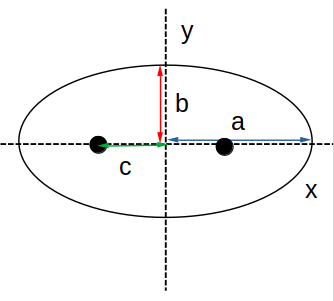
\includegraphics[width=5cm]{ellipsens_geometri.png}
    \caption{Ellipsens geometri}
\end{figure}
\end{ankiflashcard}

% DONOTREMOVE ANKI-FLASHCARD GUID 1698252197
\begin{ankiflashcard}{Formulera Keplers 3:e lag}
\underline{\textbf{Keplers 3:e lag:}} omloppstiden $\tau$ kring en kropp med massan $M$ förhåller sig till omloppsbanans halva storaxel $a$ enligt
$$
\tau = 2\pi \frac{a^{3/2}}{\sqrt{GM}}
$$
\end{ankiflashcard}

% DONOTREMOVE ANKI-FLASHCARD GUID 1284106247
\begin{ankiflashcard}{Formulera några trevliga följdsamband för Keplers tredje lag}
$\implies$ \textit{Trevliga följdsamband}:
\begin{itemize}
    \item $\tau \propto a^{3/2}$
    \item $\tau \propto (\frac{1}{E})^{3/2}$ (se \textit{Banenergi kopplat till storaxelns längd})
\end{itemize}
\end{ankiflashcard}
\ruler
\subsection{Mall för olika typer av svängingar}
Differentialekvationen för de olika svängningarna är på formen:

% DONOTREMOVE ANKI-FLASHCARD GUID 1634400825
\begin{ankiflashcard}{Ange basekvationerna för odämpade svängingar}
    
\paragraph{Odämpad svängning}
$$\ddot x + \frac{k}{m} x = \ddot x+\omega_n^2 x=\begin{cases}
\frac{F_0}{m} \sin \omega t \quad\text{om påtvingad}\\
0 \quad\text{om fri}
\end{cases}
$$
\end{ankiflashcard}

% DONOTREMOVE ANKI-FLASHCARD GUID 1676695261
\begin{ankiflashcard}{Ange basekvationerna för dämpade svängingar}
\paragraph{Dämpad svängning}
$$\ddot x + \frac{k}{m} x +  \frac{c}{m} \dot x = \ddot x+\omega_n^2 x+2\zeta \omega_n \dot x=\begin{cases}
\frac{F_0}{m} \sin \omega t \quad\text{om påtvingad}\\
0 \quad \text{om fri}
\end{cases}$$
\end{ankiflashcard}

% DONOTREMOVE ANKI-FLASHCARD GUID 1442081110
\begin{ankiflashcard}{Skriv upp formler för påtvingade svängningar}
    \subsection{Amplitud för påtvingade svängningar}
    Om en svängning påverkas av en kraft $\frac{F_0}{m}\sin/\cos \omega t$ gäller (amplituden $X$ är...):
    \begin{itemize}
        \item \textbf{Påtvingad, odämpad svängning: }$$X=\frac{F_0/k}{1-(\omega/\omega_n)^2}$$
        \item \textbf{Påtvingad, dämpad svängning: }$$X=\frac{F_0/k}{\sqrt{\left[1-(\omega/\omega_n)^2\right]^2+4\zeta^2(\omega/\omega_n)^2}}$$
    \end{itemize}
    Fullständiga partikulärlösningen: $x_p=X\sin / \cos \omega t$
\end{ankiflashcard}

% DONOTREMOVE ANKI-FLASHCARD GUID 1149215671
\begin{ankiflashcard}{När ökar amplituden för påtvingade svängningar obegränsat?}
    \subsection{Kritisk frekvens för påtvingade svängningar}
    Om $\omega = \omega_n$ kommer amplituden öka obegränsat. Om en uppgift frågar efter den ``kritiska`` amplituden är det detta som avses!
\end{ankiflashcard}

% DONOTREMOVE ANKI-FLASHCARD GUID 1913467934
\begin{ankiflashcard}{Definera förstorningsfaktor}
    Med svängningarnas amplitud $X$ kan förstoringsfaktorn (hur mycket amplituden ökar jämfört med jämviktsläget om en konstant kraft skulle inverka) defineras som
    $$M=\frac{X}{X|_{\omega=0}}$$.
\end{ankiflashcard}
\end{paracol}
\newpage
\begin{appendix}
\appendixpage
\section{Astronomisk ordlista}
\begin{itemize}
    \item 
\end{itemize}

% DONOTREMOVE ANKI-FLASHCARD GUID 1503017280
\begin{ankiflashcard}{Ange additionsformler för sinus och cosinus}
    \section{Sinus- och cosinusadditionsformler}
    Förekommer då och då i uppgifter, därför relevant att kunna dessa.
    $$\sin(\alpha\pm\beta)=\sin \alpha \cos \beta \pm \cos \alpha \sin \beta$$
     $$\cos(\alpha\pm\beta)=\cos \alpha \cos \beta \pm \sin \alpha \sin \beta$$
\end{ankiflashcard}
\end{appendix}
\end{document}
